% !TeX root = ../main.tex

\section{Results and Discussion}\label{sec:4}


In this chapter, we will discuss the results of the simulation experiments we described in Chapter 3. Table \ref{tab:result} shows the best results from the 144 experiments on the test dataset between these three learning approaches.


The complete experiment results and a link to the source code can be found in Appendix A. 

\begin{table}[!htbp]
\centering
\begin{tabular}{l|ll|ll}
\toprule
\multicolumn{1}{c|}{}       & \multicolumn{2}{c|}{Molecular Dataset}                & \multicolumn{2}{c}{Bioinformatics Dataset}           \\ \cline{2-5} 
\multicolumn{1}{c|}{Method} & \multicolumn{1}{c}{MUTAG} & \multicolumn{1}{c|}{NCI1} & \multicolumn{1}{c}{DD} & \multicolumn{1}{c}{PROTEINS} \\ \midrule
(1)\,10$\%$ SimCLR                 & 100.0$\pm$0.00             & 74.47$\pm$ 1.45            & 84.36$\pm$4.02           & 76.88$\pm$2.45                \\
(2)\,10$\%$ Barlow Twins           & 94.00$\pm$3.54              & 72.12$\pm$0.82              & 79.94$\pm$2.99           & 83.20$\pm$1.31                \\
(3)\,10$\%$ Simsiam                & 95.00$\pm$0.00              & 73.70$\pm$0.38              & 78.21$\pm$2.76           & 75.29$\pm$2.10                \\ \midrule
(4)\,10$\%$ baseline               & \multicolumn{1}{c}{-}     & 73.72$\pm$0.24              & 73.56$\pm$0.41           & 70.40$\pm$1.54                \\
(5)\,10$\%$ Aug.                   & \multicolumn{1}{c}{-}                         & 73.59$\pm$0.32              & 74.30$\pm$0.81           & 70.29$\pm$0.64                \\
(6)\,10$\%$ GAE                    & \multicolumn{1}{c}{-}                         & 74.36$\pm$0.24              & 74.54$\pm$0.68           & 70.51$\pm$0.17                \\
(7)\,10$\%$ Infomax                & \multicolumn{1}{c}{-}                        & 74.86$\pm$0.26              & 75.78$\pm$0.34           & 72.27$\pm$0.40  
\\
\bottomrule
\end{tabular}
\vspace{0.5cm}
\caption[A summary of experimental results in three learning approaches]{\textbf{A summary of experimental results for three learning approaches.} Each value in the table represents the best average of accuracy (unit: percentage) and the standard deviation in the testing stage. Results (1)–(3) are obtained from our experiments, and for Results (4)–(7), refer to You et al. \cite{GraphCL}}
		\label{tab:result}
\end{table}



\subsection{Batch size's effects on SimCLR are not apparent}

The authors of SimCLR \cite{SimCLR} pointed out that contrastive learning benefits more from a larger batch size and longer training time. They used different batch sizes, 256, 512, 1024, 2048, 4096, and 8192, to train a ResNet-50 model. They found that these batch sizes are positively correlated with the model's performance, i.e., the larger the batch size, the better the performance of the model. This concept inspires subsequent self-supervised methods to attempt to use larger batch sizes for achieving better performance. 


However, owing to computational power constraints, we only used 64 and 512 batch sizes (notice that DD uses 64 and 128). In addition, the sizes of the datasets we used are not large. The datasets contain less than 10,000 samples for model training. This makes the effect of the batch size less obvious in the SimCLR method. 


In Figure \ref{fig:simclrbatch}, the results of the experiment are separated into two categories with two batch sizes. Each point represents the accuracy of supervised learning using different parameters. The performance of two batch sizes in SimCLR is compared, and the difference is not significant.

From the above results, we can infer that the advantage of large batch sizes in contrastive learning, especially in the SimCLR model, may only be appreciable when the dataset is large. If the dataset is of medium or small size,  increasing the batch size may not improve model performance in self-supervised learning. Researchers could focus on other experiment factors.


\begin{figure}[htbp]
 
\centering
% \caption{Molecular Dataset\label{subfig:simclrbatch_mol}}
    {%
        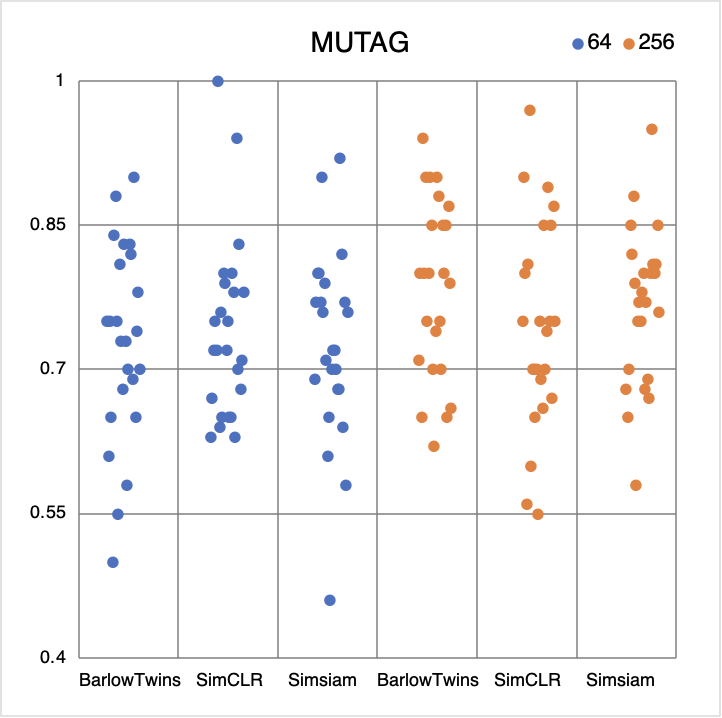
\includegraphics[width = .48\linewidth]{./figures/3-MUTAG.png}\quad
        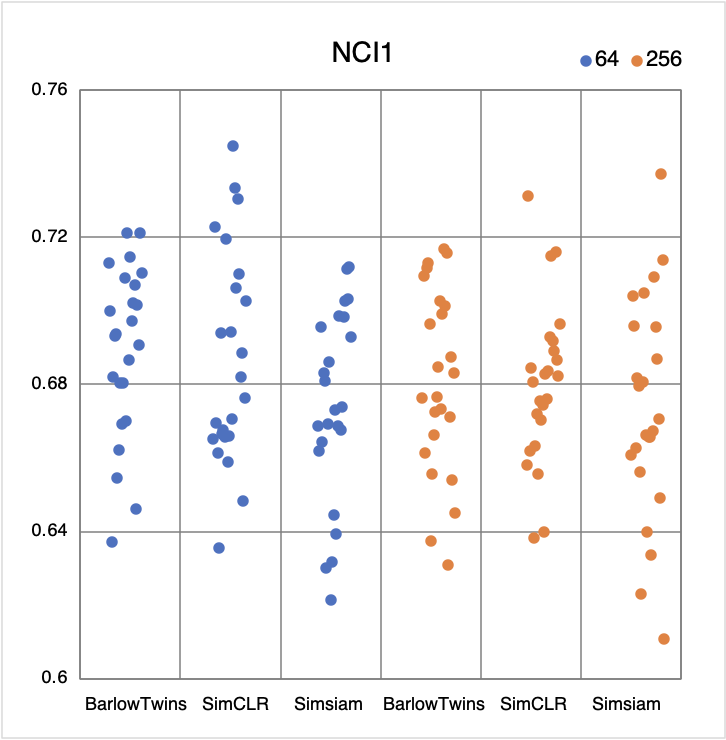
\includegraphics[width = .48\linewidth]{./figures/3-NCI1.png}}
% \caption{Bioinformatics Dataset\label{subfig:simclrbatch_bio}}
    {%
        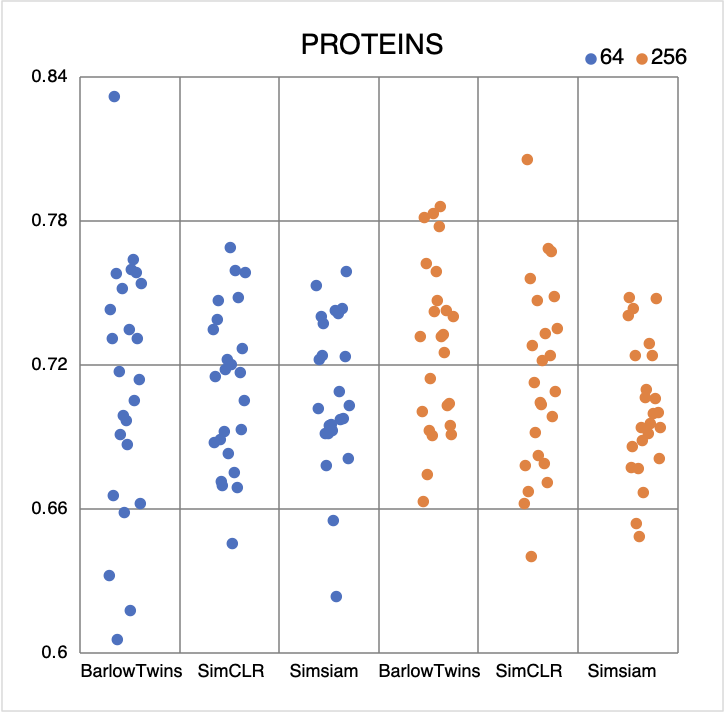
\includegraphics[width = .48\linewidth]{./figures/3-PROTEINS.png}\quad
        % \subcaptionbox{below\label{subfig:below}}
        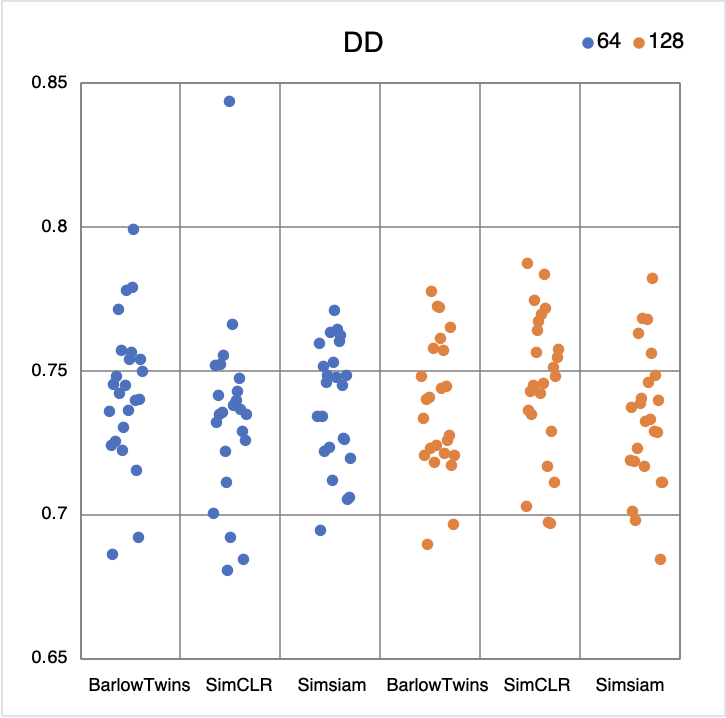
\includegraphics[width = .48\linewidth]{./figures/3-DD.png}}
\vspace{0.5cm}
\caption[Evaluation using different batch sizes]{\textbf{Evaluation using different batch sizes.} In this figure, each colored dot represents the average accuracy of experiment after five times repetitions. By grouping experiments that use the same batch sizes, we use blue and orange colors to indicate the effect of different batch sizes in different types of models. For example, in the leftmost column of each figure, the blue dots represent the performance of a model that uses Barlow Twins and 64 mini-batches.} \label{fig:simclrbatch}
\end{figure}





%%%%%%%%%%%%%%%%%%%%%%%%%%%%%%%%%%%%%%%%%%%%%%%%%%%%%%%%%%%%%%%%
%%%%%%%%%%%%%%%%%%%%%%%%%%%%%%%%%%%%%%%%%%%%%%%%%%%%%%%%%%%%%%%%
%%%%%%%%%%%%%%%%%%%%%%%%%%%%%%%%%%%%%%%%%%%%%%%%%%%%%%%%%%%%%%%%




\subsection{Deeper encoders have better performance}

Generally, models using a deep encoder are thought to have better performance than others using a shallow encoder. To judge this idea on graph datasets, we have tested three types of encoders, namely, monolayer, bilayer, and trilayer, during the training stage. 

For an encoder with a monolayer, the MLP part consists of a linear layer, followed by a ReLU layer and another linear layer. We used a graph isomorphism network encoder to generate embeddings of samples. For bilayer and trilayer architectures, the MLP parts consist of several monolayers stacked and connected by batch normalization layers.

Figure \ref{fig:deeper} shows that the medians and quartiles of accuracy are higher for models with deeper encoders. Such superior performance is particularly obvious when models are trained on the MUTAG, NCI1, and PROTEINS datasets.


Following the experiment results, the hypothesis that the deeper encoder also benefits from the graph-structured model is verified through the analysis. Future self-supervised methods should concentrate on the deeper architecture.


\begin{figure}[htbp]
\centering
% \subcaptionbox{Molecular Dataset\label{subfig:deeper_mol}}
    {%
        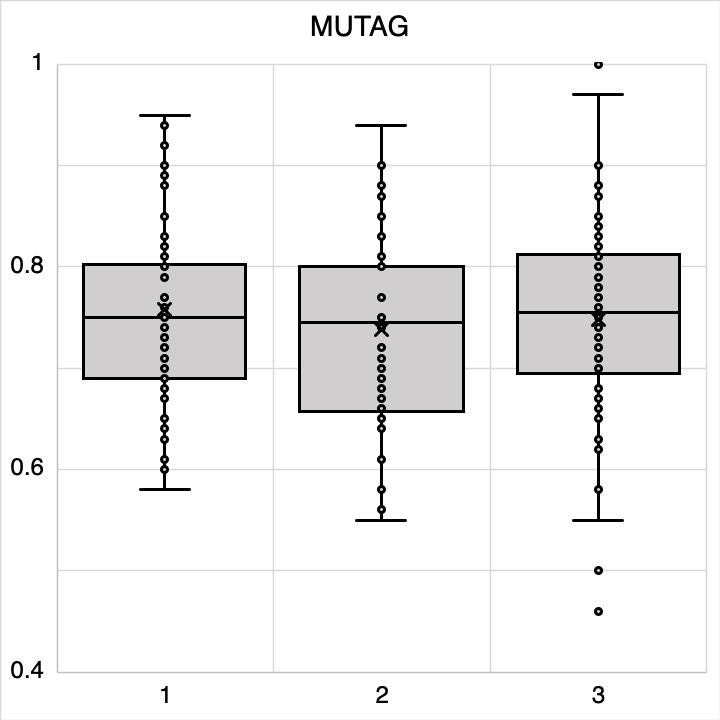
\includegraphics[width = .48\linewidth]{./figures/4-MUTAG.png}\quad
        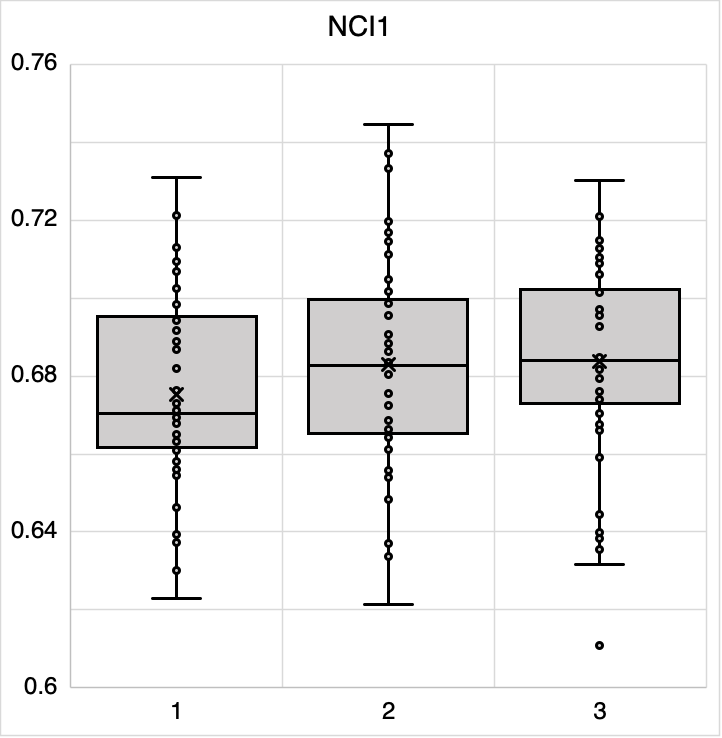
\includegraphics[width = .48\linewidth]{./figures/4-NCI1.png}}
% \subcaptionbox{Bioinformatics Dataset\label{subfig:deeper_bio}}
    {%
        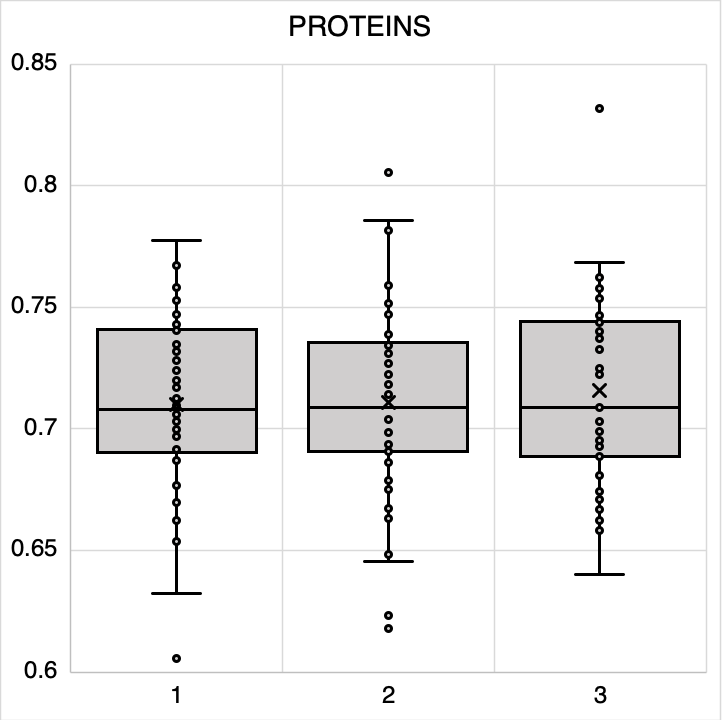
\includegraphics[width = .48\linewidth]{./figures/4-PROTEINS.png}\quad
        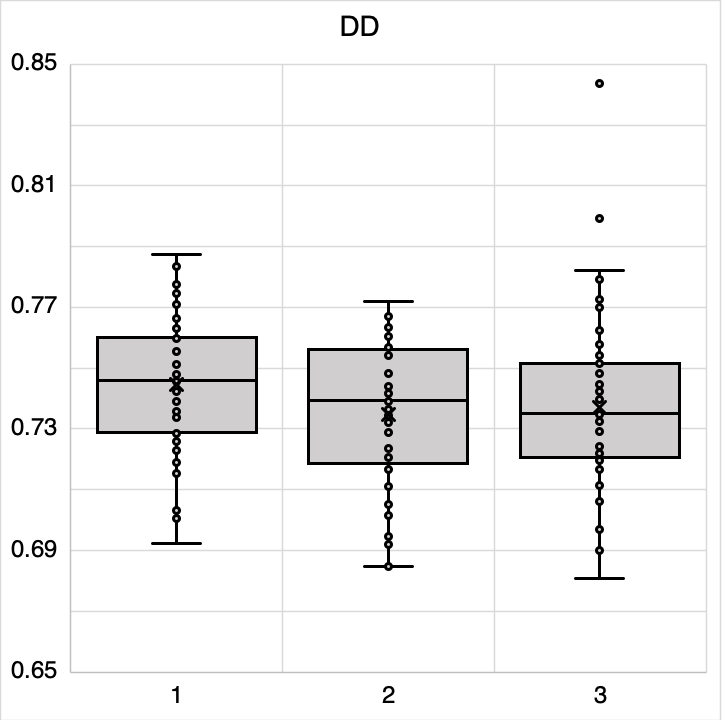
\includegraphics[width = .48\linewidth]{./figures/4-DD.png}}
\vspace{0.5cm}
\caption[Evaluation using different depths of an encoder layer]{\textbf{Evaluation using different depths of an encoder layer.} In this figure, each gray dot represents the average accuracy of experiment after five times repetitions. By grouping experiments that use the same depths of the encoder layer, we can observe the minimum, median, maximum, and quartile performance under different encoder depths. For example, in the leftmost column of each figure, the gray nodes represent the performance of a model that uses used a monolayer encoder.}\label{fig:deeper}
\end{figure}


%%%%%%%%%%%%%%%%%%%%%%%%%%%%%%%%%%%%%%%%%%%%%%%%%%%%%%%%%%%%%%%%
%%%%%%%%%%%%%%%%%%%%%%%%%%%%%%%%%%%%%%%%%%%%%%%%%%%%%%%%%%%%%%%%
%%%%%%%%%%%%%%%%%%%%%%%%%%%%%%%%%%%%%%%%%%%%%%%%%%%%%%%%%%%%%%%%


\subsection{Hidden dimension has little effect on model performance}



In most state-of-the-art neural networks, especially in image processing, NLP, and classification tasks, the hidden dimension of each encoder layer influences model performance. The hidden dimension determines the size of the feature vector. As the hidden dimension increases, an encoder can capture more complex features as hidden states, resulting in a more comprehensive representation of data.

However, in our experiment, we tested 64 and 512 hidden dimensions for models trained on the MUTAG, NCI1, and PROTEINS and tested 64 and 128 for models trained on the DD dataset. Figure \ref{fig:hidden} shows that accuracy varies across different hidden dimensions. For models with 512 hidden dimensions, even if the vector size is eight times larger than those with 64 hidden dimensions, there is no significant improvement in model performance. 


These surprising differences can be explained in part by the data structure of graph and image data. For image data, which consist of discrete pixels, with a larger hidden dimension, a neuron can capture more information via pixel clustering. However, graph data are more abstract. Nodes and edges cannot be separated or unified as pixel groups in image data. This difference makes adding hidden dimensions less effective in model training. 

In summary, if we want to apply a self-supervised method to graph data, increasing the hidden dimension size may not be helpful. However, if the raw data can be discretization into small units, such as an image into pixels, or a sentence into n-gram, increasing the hidden dimension size is a reliable way to improve performance. 


\begin{figure}[htbp]
\centering
% \subcaptionbox{Molecular Dataset\label{subfig:hidden_mol}}
    {%
        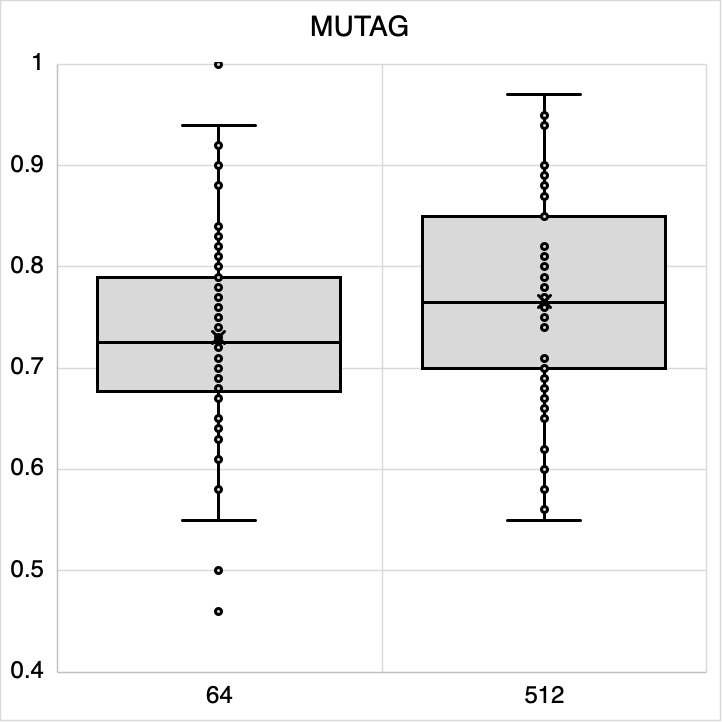
\includegraphics[width = .48\linewidth]{./figures/5-MUTAG.png}\quad
        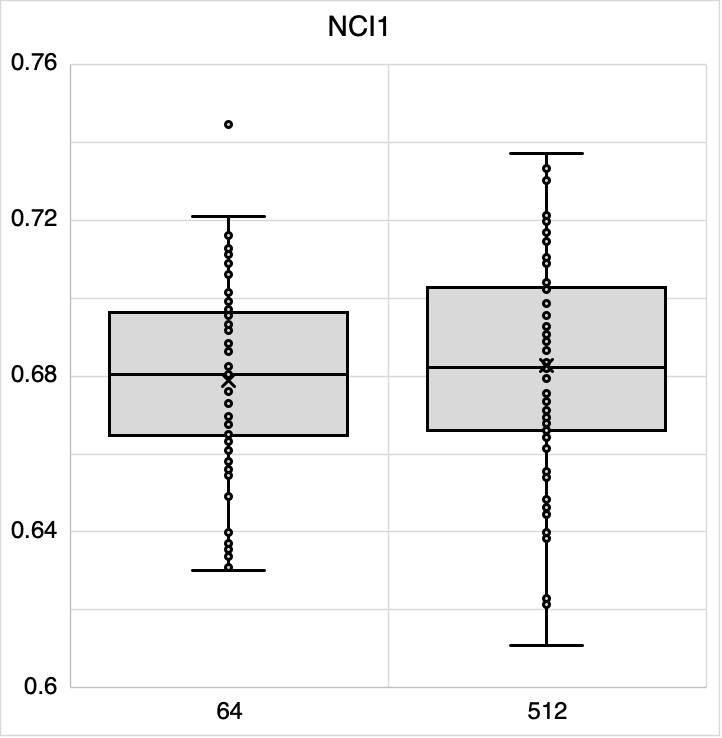
\includegraphics[width = .48\linewidth]{./figures/5-NCI1.png}}
% \subcaptionbox{Bioinformatics Dataset\label{subfig:hidden_bio}}
    {%
        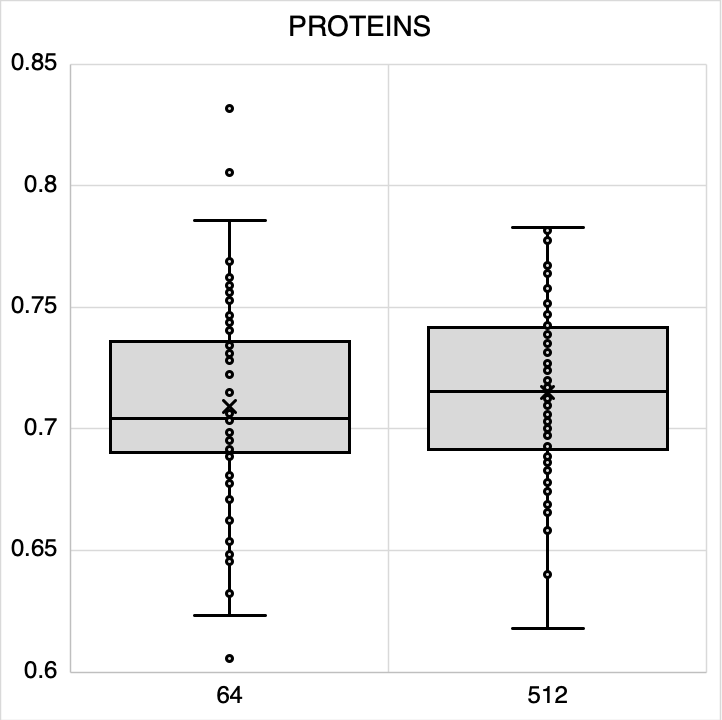
\includegraphics[width = .48\linewidth]{./figures/5-PROTEINS.png}\quad
        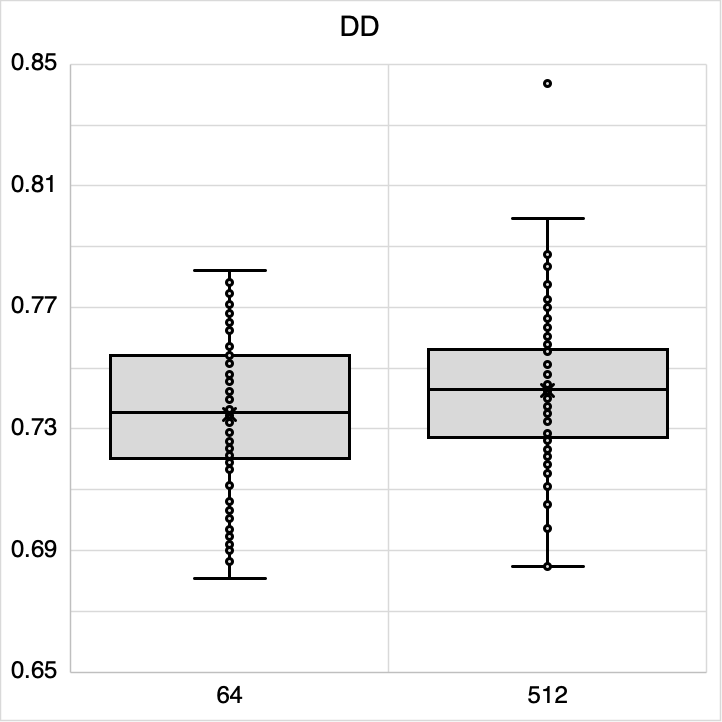
\includegraphics[width = .48\linewidth]{./figures/5-DD.png}}
\vspace{0.5cm}
\caption[Evaluation using different hidden dimensions]{\textbf{Evaluation using different hidden dimensions.} In this figure, each gray dot represents the average accuracy of experiment after five times repetitions. By grouping experiments that use the same hidden dimensions, we can observe the minimum, median, maximum, and quartile performance under different hidden dimensions in the hidden layer. For example, in the leftmost column of each figure, the gray dots represent the performance of a model that uses 64 hidden dimensions.}\label{fig:hidden}
\end{figure}


%%%%%%%%%%%%%%%%%%%%%%%%%%%%%%%%%%%%%%%%%%%%%%%%%%%%%%%%%%%%%%%%
%%%%%%%%%%%%%%%%%%%%%%%%%%%%%%%%%%%%%%%%%%%%%%%%%%%%%%%%%%%%%%%%
%%%%%%%%%%%%%%%%%%%%%%%%%%%%%%%%%%%%%%%%%%%%%%%%%%%%%%%%%%%%%%%%


\subsection{SimCLR performs better in molecular datasets}


In our experiments, we used four datasets, of which two, MUTAG and NCI1, are molecular datasets. The other two datasets, PROTEINS and DD, are bioinformatics datasets. Figure \ref{fig:simclrbetter} shows that models trained via SimCLR performed better than models trained via the other approaches on both molecular datasets. Conversely, models trained via SimCLR did not outperform models trained via Barlow Twins and Simsiam on bioinformatics datasets.


Reviewing these datasets will help us understand why performance varies. Although these data are graph-structured, there are fundamental differences between molecular and bioinformatics graph data. In molecular datasets, e.g., MUTAG and NCI1, each node represents an atom, and each edge represents a chemical bond connecting two nodes. In bioinformatics datasets, such as PROTEINS and DD, each node represents an amino acid, and two nodes are connected by an edge if they are less than 6 angstroms apart.

Both types of datasets have different types of properties, which can have complex effects on self-supervised models. Unlike Simsiam that only uses one projection, or Barlow Twins that uses embeddings directly, in the SimCLR architecture, raw data and augmented data are encoded into projections, which may affect performance.

The experimental results indicate that SimCLR is a suitable application model for molecular datasets; however, more empirical experiments are required to verify its robustness. Unfortunately, at present, owing to computational power constraints, this study lacks experimental logs of larger molecular datasets. A further study focusing on SimCLR or molecular graph-structured datasets should be conducted.


\begin{figure}
\centering
% \subcaptionbox{Molecular Dataset\label{subfig:simclrbetter_mol}}
    {%
        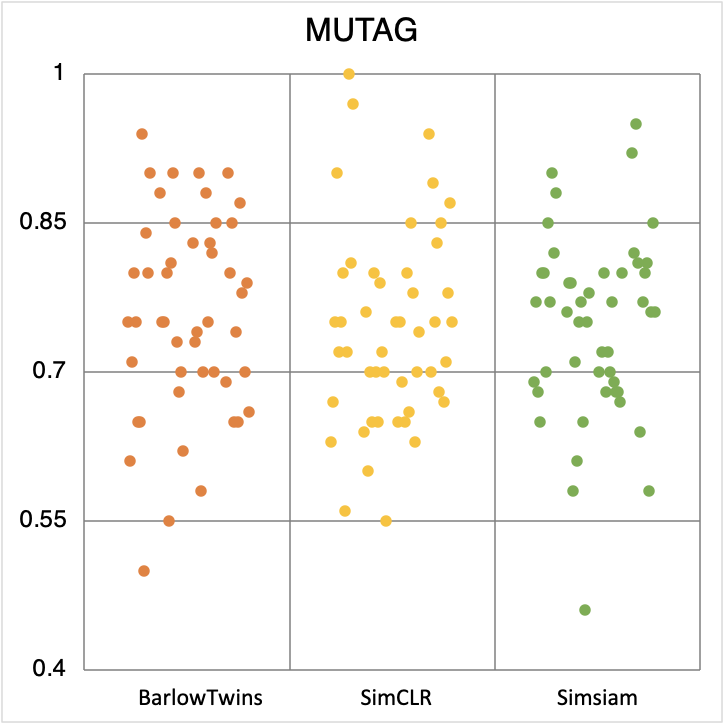
\includegraphics[width = .48\linewidth]{./figures/1-MUTAG.png}\quad
        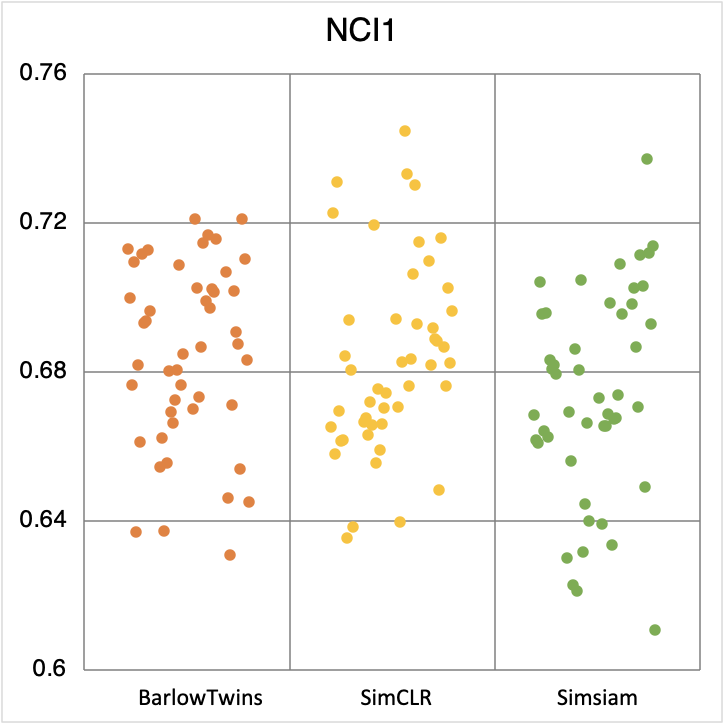
\includegraphics[width = .48\linewidth]{./figures/1-NCI1.png}}
% \subcaptionbox{Bioinformatics Dataset\label{subfig:simclrbetter_bio}}
    {%
        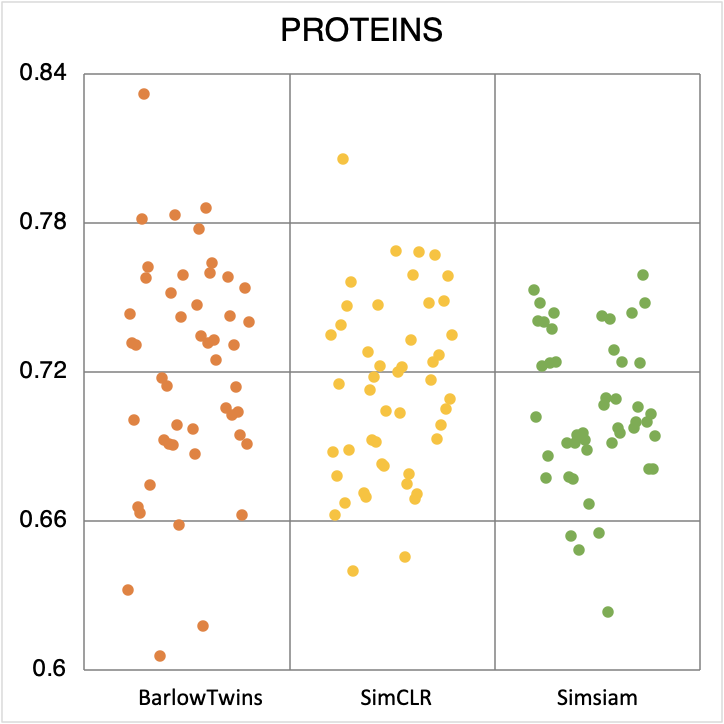
\includegraphics[width = .48\linewidth]{./figures/1-PROTEINS.png}\quad
        % \subcaptionbox{below\label{subfig:below}}
        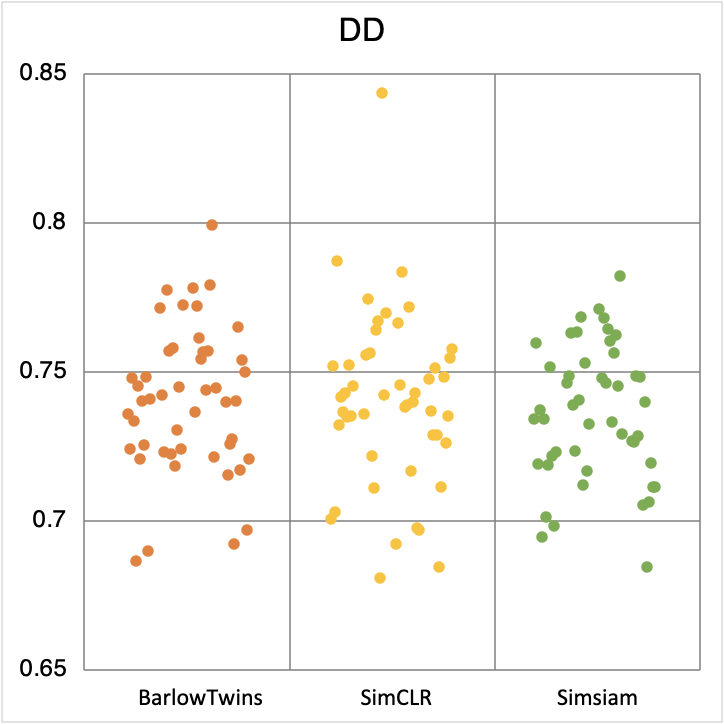
\includegraphics[width = .48\linewidth]{./figures/1-DD.png}}
\vspace{0.5cm}
\caption[Evaluation using different self-supervised methods]{\textbf{Evaluation using different self-supervised methods.} In this figure, each colored dot represents the average accuracy of experiment. By grouping experiments that use the same approaches, we use orange, yellow, and green colors to indicate the evaluation via Barlow Twins, SimCLR, and Simsiam, respectively. For example, in the leftmost column of each figure, the orange dots represent the performance of a model that uses Barlow Twins.}
\label{fig:simclrbetter}
\end{figure}


%%%%%%%%%%%%%%%%%%%%%%%%%%%%%%%%%%%%%%%%%%%%%%%%%%%%%%%%%%%%%%%%
%%%%%%%%%%%%%%%%%%%%%%%%%%%%%%%%%%%%%%%%%%%%%%%%%%%%%%%%%%%%%%%%
%%%%%%%%%%%%%%%%%%%%%%%%%%%%%%%%%%%%%%%%%%%%%%%%%%%%%%%%%%%%%%%%

\subsection{SUBGRAPH augmentation performs closer in bioinformatics dataset}


Furthermore, there is an interesting discovery in our experiment results. The idea behind data augmentation, especially in the SUBGRAPH operator, assumes that the partial graph should retain the properties of the entire graph, even when some nodes or edges are added or removed.  

From Figure \ref{fig:stable} shows that models trained using the SUBGRAPH operator achieve similar performance on the DD and PROTEINS datasets. The variance in performance was lower than those on the molecular datasets.



As previously mentioned, molecular and bioinformatics datasets have different properties and targets. First, the goal of MUTAG is to train models to predict the mutagenicity of Salmonella typhimurium. Second, the goal of NCI1 is to train models to classify whether a chemical compound is positive or negative for cell lung cancer. Third, the goal of the PROTEINS and DD datasets is to train models to predict which proteins are enzymes or non-enzymes.

In a chemical molecule, each node and edge play a unique role. The functional group may be lost if we only capture a part of the graph. For example, the chemical formula of ethanol (a.k.a. alcohol) is $\text{C}_{2}\text{H}_{5}\text{OH}$, containing a hydroxyl group (-OH). If the augmented operator samples $\text{C}_{2}\text{H}_{4}$, it will be recognized as ethene, which has different chemical properties from ethanol. Because the augmented data have more diversity, the performance of the model will have a higher variance.


In contrast, a protein contains at least one long polypeptide, which is chained by amino acid. Proteins can be constructed in flexible ways \cite{accurateprotein}. Some proteins chained by different polypeptides can have similar chemical properties and functions. Therefore, even when we use the SUBGRAPH operator, the augmented data are similar to the raw data, reducing the variance between experiment results.



This finding, while preliminary, suggests that augmented data generated using the SUBGRAPH operator should be carefully used. To avoid a good experiment result producing trivial analysis, we should first observe the representation of each node and edge and consider their chemical and physic attributes before attempting to sample raw data as augmentation data.

\begin{figure}
\centering
% \subcaptionbox{Molecular Dataset\label{subfig:stable_mol}}
    {%
        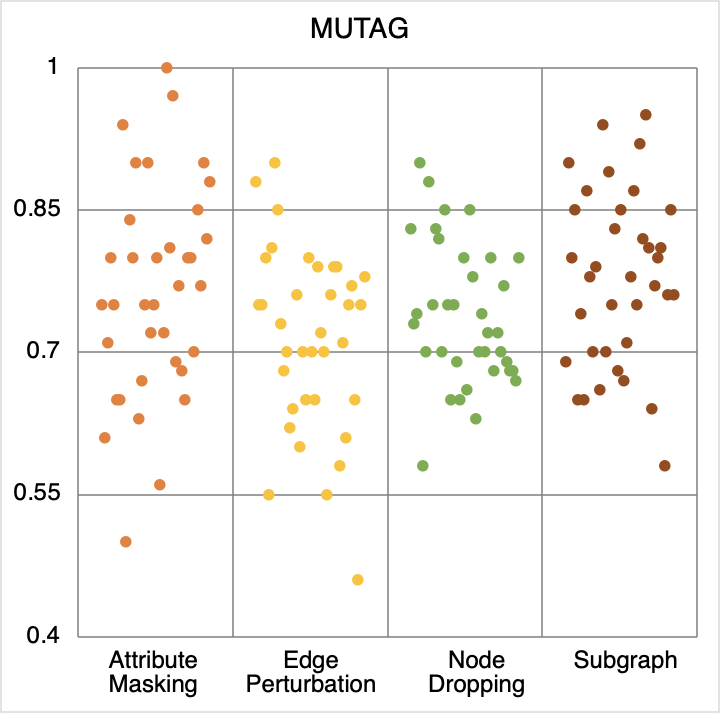
\includegraphics[width = .48\linewidth]{./figures/2-MUTAG.png}\quad
        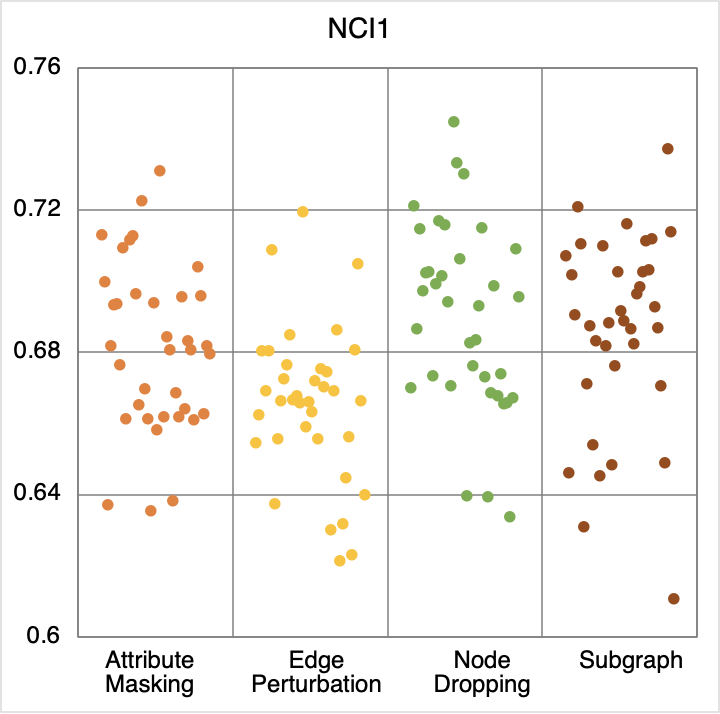
\includegraphics[width = .48\linewidth]{./figures/2-NCI1.png}}
% \subcaptionbox{Bioinformatics Dataset\label{subfig:stable_bio}}
    {%
        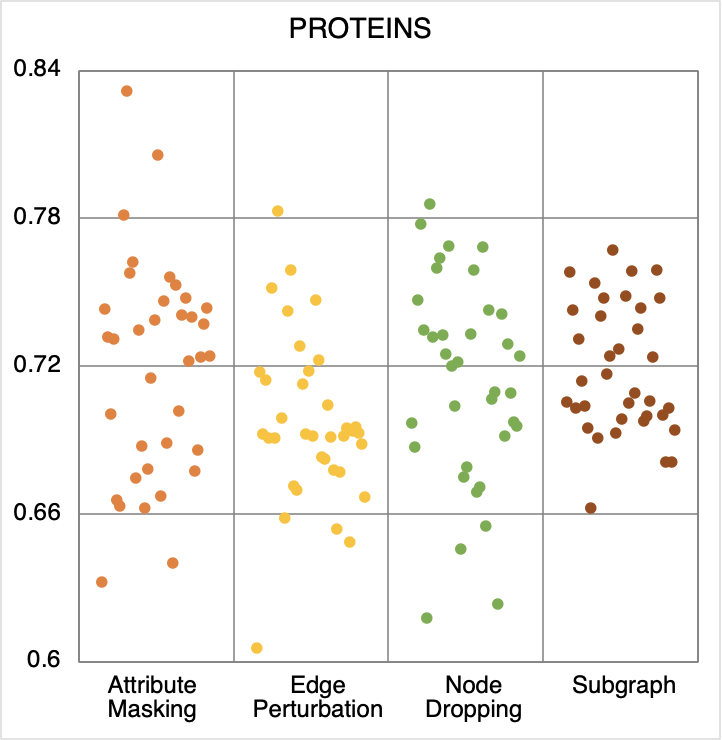
\includegraphics[width = .48\linewidth]{./figures/2-PROTEINS.png}\quad
        % \subcaptionbox{below\label{subfig:below}}
        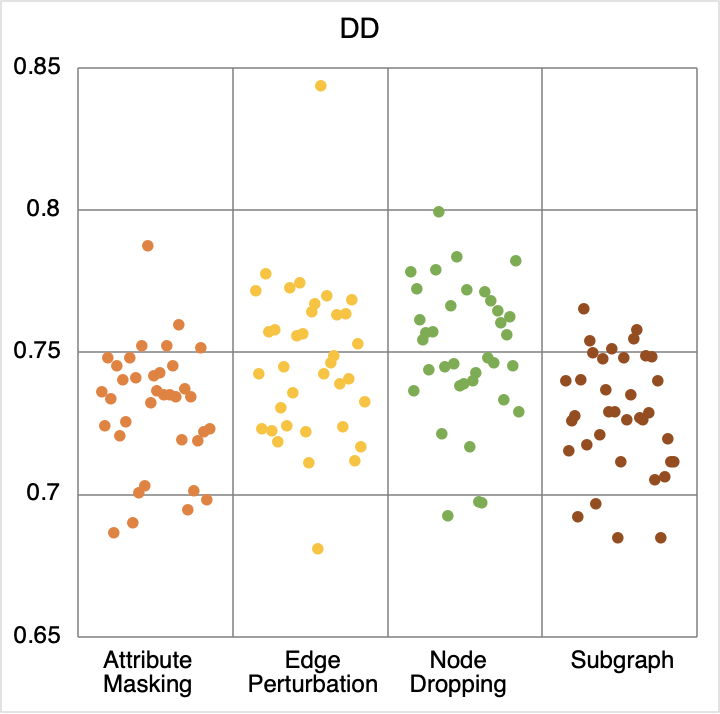
\includegraphics[width = .48\linewidth]{./figures/2-DD.png}}
\vspace{0.5cm}
\caption[SUBGRAPH augmentation performs better on bioinformatics datasets]{\textbf{SUBGRAPH augmentation performs better on bioinformatics datasets.} In this figure, each colored dot represents the average accuracy of experiment. By grouping experiments that use the same data augmentation method, we use orange, yellow, green, and brown colors to indicate the evaluation by ATTRIBUTE MASKING, EDGE PERTUBATION, NODE DROPPING, and SUBGRAPH, respectively. For example, in the leftmost column of each figure, the orange dots represent the performance of a model that uses ATTRIBUTE MASKING to generate augmented data.}
\label{fig:stable}
\end{figure}


%%%%%%%%%%%%%%%%%%%%%%%%%%%%%%%%%%%%%%%%%%%%%%%%%%%%%%%%%%%%%%%%
%%%%%%%%%%%%%%%%%%%%%%%%%%%%%%%%%%%%%%%%%%%%%%%%%%%%%%%%%%%%%%%%
%%%%%%%%%%%%%%%%%%%%%%%%%%%%%%%%%%%%%%%%%%%%%%%%%%%%%%%%%%%%%%%%


\subsection{Discussion}

Most studies on self-supervised learning have only been conducted in image processing and NLP. In this chapter, we have revised the properties of graph data, analyzed the experimental results, and attempted to provide some possible explanations. 

According to our findings, not all hyperparameters influence model performance significantly. Some of them only have a small effect when the dataset size is not sufficiently large. On the other hand, the fundamental differences between graphs and other data structures, along with the categories of graph datasets, prevent models from applying the same training strategies.